\chapter{Related Work}\label{chapter:related_work}
This work is not the first to explore the area of code-generation and  compiling regular expressions. In 2008, \citet{firejpaper} implemented FIRE/J (Fast Implementation of Regular Expressions for Java) which is a portable POSIX compatible Java regular expression library that focuses on providing maximum regex matching speed. In their implementation, they converted the regular expression into a DFA that is again compiled directly into Java source code or JVM Bytecode.

\noindent FIRE/J generated byte-code shown in Figure \ref{fig:firejpaper} is similar in structure of our generated LLVM IR. The algorithm lists each DFA state starting from the initial state then the input characters checked against the transition rules of the DFA states. If a character does not satisfy the selected state, then the match fails. While their approach is similar to ours there are a few difference between them and ours mainly (1) their use-case is to be used as a generic java library while ours is usage as a sub-engine inside a database. (2) The execution and compilation speed of LLVM compiler infrastructure is far superior to traditional JVM byte-code that Azul JVM implementation based on LLVM is 5 to 250 percent faster than Oracle's HotSpot Java platform \cite{azul}.

PCRE2 is a regular expressions matching library for the C programming language. This library translates the patterns into byte-code that can be executed by its interpreter.  In 2016, \citet{pcre2_jit} developed a new backtracking based matching algorithm for PCRE2 called \textit{static-backtracking} and a JIT compiler for PCRE2 called \textit{PCRE-JIT}.

Static backtracking algorithm generates machine code from the Abstract Syntax Tree (AST). The AST representation provides more information about the pattern's structure and allows the engine to optimize both matching and backtracking simultaneously rather than focusing only on matching. The PCRE-JIT compiler transforms PCRE byte-code into low-level intermediate representation (LIR) language of the Stackless Just-In-Time Compiler (SLJIT), which then translates it into machine code. In Chapter \ref{chapter:evaluation}, We compare our DFA-based engine performance to that of PCRE-JIT.

ReJit \cite{rejit} is an is a prototype of a non-backtracking, just-in-time, SIMD-able regular expression engine. ReJit generates tailored machine code to match each regular expression, that is passed to a JIT compiler that enables identifying what CPU instructions are available at run-time and creating efficient code for performance-critical areas.

Despite being based on Finite Automaton, It supports the vast majority of regular expression capabilities (including some that RE2 does not, such as back-references). To handle back-references, Backtracking is used locally for them and not as a general algorithm.

When Matching complex regular expressions, Most engines will try to match the regexps from the start, which might be wasteful. ReJit on the other hand, tries to find the easy section of the regexps first and then complete the match from there. E.g. for the pattern \texttt{\textbf{[0-9]{3,10}\%foo\%[A-Za-z]}}, it generates code that first searches for \texttt{\textbf{foo}} and then proceeds backward and forward to match the entire phrase.

ReJit is a promising engine but is still a work-in-progress. It currently only supports \texttt{\textbf{X86}} CPU architecture. It is also not in active development since 2015 (time of the last commit \footnote{\url{https://github.com/coreperf/rejit/commit/36855db0644d6f3dbad69dc65cf002c81510ea19}}).

\begin{figure}[H]
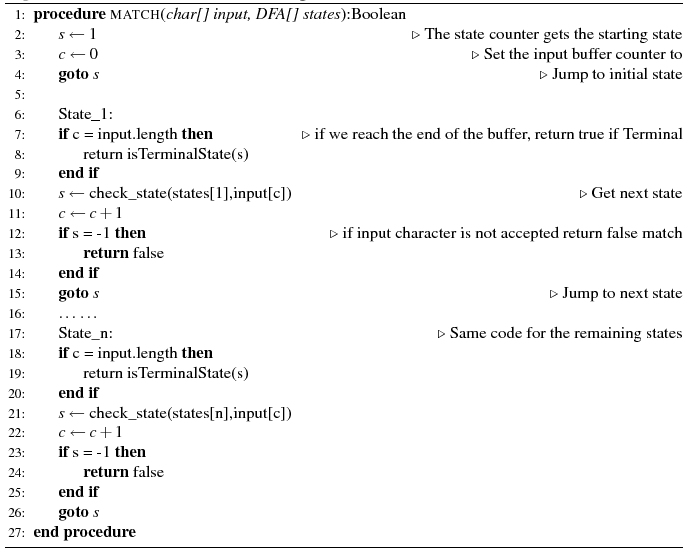
\includegraphics[width=0.85\textwidth]{imgs/alg-byte-firej.png}
\caption{FIRE/J \cite{firejpaper} Generated Byte-code.}\label{fig:firejpaper}
\end{figure}


\citet{simdregextpch} in their paper SIMD-Accelerated Regular Expression Matching, presented the design and implementation of SIMD-vectorized regular expression matching for filtering DBMSs string columns. 

In their approach, they processes multiple input strings in a data-parallel way that avoids reading the strings in lockstep without branching in order to exploit scenarios when some strings are accepted or rejected early by inspecting the first few characters. Their approach achieved up to $2x$ speedup on a mainstream CPU and $5x$ speedup on the Xeon Phi co-processor using common string lengths.


\citet{parabixorg} introduced Parabix (Parallel Bit Streams) a generic framework and toolkit describing the software toolchain and run-time support that enables applications to use modern SIMD instructions for high-performance text processing.

Parabix exploits data-level parallelism of wide SIMD registers to implement parallel bit streams through the use of bitwise data parallelization. In 2014, \citet{parabixregexnew} developed a new algorithm and compiler that utilize using bitwise data parallelism for regular expression matching. The algorithm represents a general solution to the problem of regular expression matching utilizing parallel bit streams. The prototype compiler consisted of a tool-chain that compiled a regular expression to bit-parallel streams. The bit-stream is then compiled to highly efficient SIMD C++ code which is then compiled to machine code. The prototype did not support Unicode, it only supported ASCII.

In 2015, \citet{parabix} unified the tool-chain into a single executable compiler that is highly efficient Unicode-capable and is dynamically compiled (JITed) using the LLVM compiler infrastructure. When compared to other Unicode-capable regular expression search tools, performance evaluations reveal asymptotic performance advantages of more than 10X, while the overhead of dynamic compilation approaches restricts the benefits to rather large input files.